\documentclass[twoside]{article}

\usepackage{lipsum}
\usepackage[none]{hyphenat} 

\usepackage[sc]{mathpazo} 
\usepackage[T1]{fontenc} 
\linespread{1.05}
\usepackage{microtype}

\usepackage[hmarginratio=1:1,top=32mm,columnsep=20pt]{geometry}
\usepackage{multicol} 
\usepackage[hang, small,labelfont=bf,up,textfont=it,up]{caption} 
\usepackage{booktabs} 
\usepackage{float} 
\usepackage{hyperref}
\usepackage{amsmath}

\usepackage{lettrine} 
\usepackage{paralist}

\usepackage{abstract} 
\renewcommand{\abstractnamefont}{\normalfont\bfseries}
\renewcommand{\abstracttextfont}{\normalfont\small\itshape} 

\usepackage{titlesec} 
\renewcommand\thesection{\Roman{section}} 
\renewcommand\thesubsection{\Roman{subsection}} 
\titleformat{\section}[block]{\large\scshape\centering}{\thesection.}{1em}{} 
\titleformat{\subsection}[block]{\large}{\thesubsection.}{1em}{}

\usepackage{fancyhdr} 
\pagestyle{fancy} 
\fancyhead{} 
\fancyfoot{}

\fancyhead[C]{ SRI $\bullet$ Proyecto Final $\bullet$ C-511}
\fancyfoot[RO,LE]{\thepage}

\title{\vspace{-0.5cm}\fontsize{20pt}{10pt}\selectfont\textbf{Proyecto Final Sistemas de Recuperaci\'on de la Informaci\'on}}

\author{
\large
\textsc{\vspace{-2cm} Alejandro Campos, Darian Dominguez}\\[3.5cm]
\normalsize Facultad de Matem\'atica y Computaci\'on \\
\normalsize Universidad de la Habana \\
\normalsize 2022 \\[1cm]
\vspace{-5mm}
}
\date{}


\usepackage{graphicx}
\begin{document}

\maketitle

\thispagestyle{fancy} 

\begin{center}
\textbf{Resumen}
\end{center}
\noindent \textit{ En el mundo de hoy se tiene acceso a mucha informaci\'on. Ser\'ia muy complicado para una persona buscar, entre millones y millones de documentos, cu\'ales ser\'ian \'utiles y relevantes para su objetivo. Los sistemas de recuperaci\'on de la informaci\'on facilitan este trabajo. Estos reciben una consulta por parte del usuario y procesan toda la colecci\'on de documentos, que luego de analizarlos y representarlos de una forma que el sistema entiende, devuelven en un corto per\'iodo de tiempo aquellos archivos m\'as relevantes a la petici\'on del usuario.}\\[0.5cm]

%\begin{multicols}{2}

\section{Introducci\'on}
\qquad Realizar b\'usquedas de informaci\'on es una actividad diaria en todos los ambientes que reviste especial importancia. En \'areas de investigaci\'on es una actividad que puede insumir un tiempo importante entre operaciones que van desde: definir los criterios, iniciar la b\'usqueda, filtrar los resultados, encontrar la informaci\'on y luego tenerla a disposici\'on de una manera clasificada y ordenada. La fase de b\'usqueda se inicia sobre las expectativas planteadas por el investigador y finaliza cuando el mismo encuentra finalmente el o los documentos que poseen la informaci\'on de inter\'es. [1]

Varios documentos pueden responder a la consulta del usuario, por ello, los sistemas implementan un ranking de documentos ordenados seg\'un la relevancia a la petici\'on del usuario, dependiendo del modelo sobre los que son implementados. Existen disc\'imiles modelos para recuperar informaci\'on, estos se diferencian en la manera de representar los documentos y la consulta, en dependencia de los t\'erminos que la conforman. A partir de esta forma de representaci\'on, se le asocia a cada documento un valor calculado mendiante una funci\'on de ranking, que var\'ia en dependencia del modelo utilizado. 

Este informe tiene como objetivo describir el dise\~no, implementaci\'on, evaluaci\'on y an\'alisis de un Sistema de Recuperaci\'on de Informaci\'on.\\\\


\section{Dise\~no del sistema}
\qquad Luego del estudio y an\'alisis de los modelos estudiados en [2], se decidi\'o usar el modelo vectorial para el desarrollo del sistema de recuperaci\'on de la informaci\'on. En la presente secci\'on se explicar\'an los motivos de esta selecci\'on, no sin antes explicar en qu\'e consiste este modelo.

Brevemente, seg\'un este modelo, cada documento es representado mediante un vector de n elementos, siendo n igual al n\'umero de t\'erminos indizables que existen en la colecci\'on documental. Hay, pues, un vector para cada documento, y, en cada vector, un elemento para cada t\'ermino o palabra susceptible de aparecer en el documento. Cada uno de esos elementos es cubierto u ocupado con un valor num\'erico. Si la palabra no est\'a presente en el documento, ese valor es igual a 0. En caso contrario, ese valor es calculado teniendo en cuenta diversos factores, dado que una palabra dada puede ser m\'as o menos significativa (tanto en general como, sobre todo, en ese documento en concreto); este valor se conoce con el nombre de peso del t\'ermino en el documento. Las consultas son representadas tambi\'en mediante un vector de las mismas caracter\'isticas que las de los documentos. Esto permite calcular f\'acilmente una funci\'on de similaridad dada entre el vector de una consulta y los de cada uno de los documentos.[3]

El modelo vectorial es ampliamente usado en operaciones de recuperaci\'on de informaci\'on, as\'i como tambi\'en en operaciones de categorizaci\'on autom\'atica, filtrado de informaci\'on, etc. Aunque tiene la desventaja de asumir independencia de t\'erminos, el c\'alculo del valor asociado a cada documento para realizar el ranking se determina por la cercan\'ia de este con respecto a la consulta del usuario, definida por el coseno del \'angulo entre el vector que representa al documento y el de la consulta. Podemos decir, adem\'as, que el esquema de ponderaci\'on de este modelo (tf-idf como se ver\'a posteriormente) permite un mejor rendimiento en la recuperaci\'on de informaci\'on.\\\\

\section{Implementaci\'on del sistema}
\qquad El sistema se ha implementado usando el lenguaje de programaci\'on python, cuyas bibliotecas ofrecen facilidades para el trabajo con el procesamiento textual. La implementaci\'on se encuentra en la carpeta \textbf{code}. En las siguientes subsecciones se explica el uso de cada uno de los m\'odulos m\'as importantes del sistema.\\

\subsection{Procesamiento textual}
\qquad En el m\'odulo \texttt{text\_processing.py} se realizan todas las fases del preprocesamiento textual, tokenizaci\'on, normalizaci\'on, lematizaci\'on o reducci\'on de las palabras a su ra\'iz gramatical y eliminaci\'on de stopwords. Para esto se us\'o la librer\'ia \textit{nltk}.

\subsection{Representaci\'on de documentos y consultas}
\qquad \texttt{representation.py} provee m\'etodos para la representaci\'on de documentos y consultas. En este se calcula el $tf$ de cada t\'ermino en cada documento, as\'i como $idf$ de cada t\'ermino y, a trav\'es de estos, se determina el peso de cada t\'ermino $i$ en el documento $j$ ($w_{ij}$). Se precisan a continuaci\'on cada uno de los t\'erminos anteriores.
$$tf_{ij} = \frac{freq_{ij}}{max_i freq_{ij}}$$ donde el numerador corresponde a la cantidad de veces que se repite el t\'ermino $i$ en el documento $j$, y el denominador es la cantidad de veces que se repite el t\'ermino que m\'as se repite en el documento $j$. Tambi\'en se tiene que $$idf_i = log \frac{N}{n_i}$$ donde N corresponde a la cantidad total de documentos de la colecci\'on y $n_i$ a la cantidad de documentos en los que aparece el t\'ermino $i$. Finalmente, el peso de un t\'ermino en el documento, viene dado por $$w_{ij} = tf_{ij} * idf_i$$. Como ya se dijo, los documentos son represantados como vectores, cuyas componentes vienen dadas por los pesos de los t\'erminos que aparecen en estos.[4]

Las consultas tambi\'en son representadas como vectores, el peso de un t\'ermino en la consulta $q$ viene dado por $$w_{iq} = (a + (1 - a)tf_{ij}) * idf_i$$ donde $a$ usualmente toma valor 0.4 o 0.5 [4]. Notemos que si a = 0 el peso de la consulta es el mismo que el del documento.

\subsection{Documentos}
\qquad Las colecciones de documentos se encuentran en la carpeta "static/collections". El sistema trabajar\'a con la colecci\'on de archivos con extensi\'on .txt localizados en dicha ruta. En \texttt{document\_processing.py} se procesan todos los documentos de la colecci\'on. A sus textos se les realiza el procesamiento textual y se calcula el peso de cada t\'ermino resultante en cada documento.

\subsection{Funci\'on de similitud}
\qquad El m\'odulo \texttt{sim.py} contiene el c\'alculo de la funci\'on de similitud, mediante la cual se realiza el ranking de los  documentos. Acorde al modelo empleado, esta funci\'on se calcula como el coseno del \'angulo comprendido entre el vector que representa cada uno de los documentos y la consulta.  $$sim(d_j,q) = \frac{\vec{d_j} \vec{q}}{|\vec{d_j}||\vec{q}|},$$ esto es $$sim(dj, q) = \frac{\sum_{i=1}^n w_{ij} w_{iq}}{\sqrt{\sum_{i=1}^n w_{ij}^2}\sqrt{\sum_{i=1}^n w_{iq}^2}} \qquad \text{[4]}$$

\subsection{Procesamiento de consulta y devoluci\'on de resultados}
\qquad Al texto de la consulta se le realiza un preprocesamiento, como se expuso en la secci\'on correspondiente. Luego se le calcula el peso de cada t\'ermino para formar el vector consulta, a partir del cual la funci\'on de similitud le asocia un valor a cada documento y devuelve el ranking de estos, a partir de un umbral que se define previamente. Esto se realiza en \texttt{query\_processing.py}.

\subsection{Expansi\'on de consulta}
\qquad El sistema implementa la expansi\'on de consulta, lo cual permite expandir las consultas ingresadas por el usuario a fin de ampliar el espectro de las b\'usquedas que se realicen. El m\'odulo \texttt{query\_expansion.py} implementa esta funcionalidad, donde por cada t\'ermino $t$ de la consulta, esta es expandida autom\'aticamente con sin\'onimos y palaras relacionadas con $t$.

\subsection{Clustering}
\qquad Los documentos se agrupan seg\'un su similitud de acuerdo al contenido que presentan. El m\'odulo \texttt{clustering.py} utiliza el algoritmo k-means con este fin. De esta forma el usuario recibe la colecci\'on de documentos agrupados por t\'opicos, lo cual es de utilidad para explorar documentos similiares a los devueltos como resultado en la consulta, y explorar los documentos de aquellos temas que le resulten de inter\'es. Para seleccionar el n\'umero de clusters para agrupar los documentos se usa el m\'etodo del codo, cuya impementaci\'on se encuentra, tambi\'en, en dicho m\'odulo.

\section{Modelo booleano}
\qquad Con el fin de comparar el sistema desarrollado, se implement\'o otro modelo: el modelo booleano. Este modelo se basa en la teor\'ia de conjuntos y el \'algebra booleana para devolver los resultados [4]. En este modelo las consultas est\'an dise\~nadas como expresiones booleanas que tienen una sem\'antica precisa y, considera solo si los t\'erminos indexados est\'an presentes o ausentes en un documento. La estrategia de recuperaci\'on se basa en un criterio de decisi\'on binario.

En el m\'odulo \texttt{boolean\_model.py} se encuentra la implementaci\'on de este modelo. Luego del preprocesamiento del texto de los documentos, estos se expresan como vectores binarios atendiendo a la presencia o no de t\'erminos indexados. Posteriormente, desp\'ues del preprocesamiento y expansi\'on de la consulta, esta se convierte en una expresi\'on booleana de tal forma que si el t\'ermino $t_q$ de la consulta est\'a presente en los t\'erminos indexados, entonces la componente correspondiente al t\'ermino es 1, en otro caso toma valor 0.

Con la representaci\'on booleana abordada anteriormente, la funci\'on de similitud en este modelo devuelve aquellos documentos que "se parezcan m\'as" a la consulta, es decir, aquellos documentos que tengan m\'as componentes en com\'un con esta. 


\section{Interfaz de usuario. Manual de usuario}
\qquad Para la interfaz de usuario se us\'o la librer\'ia \textit{flask} que permite crear aplicaciones web r\'apidamente, usando html, css y javascript.

Al abrir la aplicaci\'on se mostrar\'a la pantalla de presentaci\'on como se muestra a continuaci\'on:\\

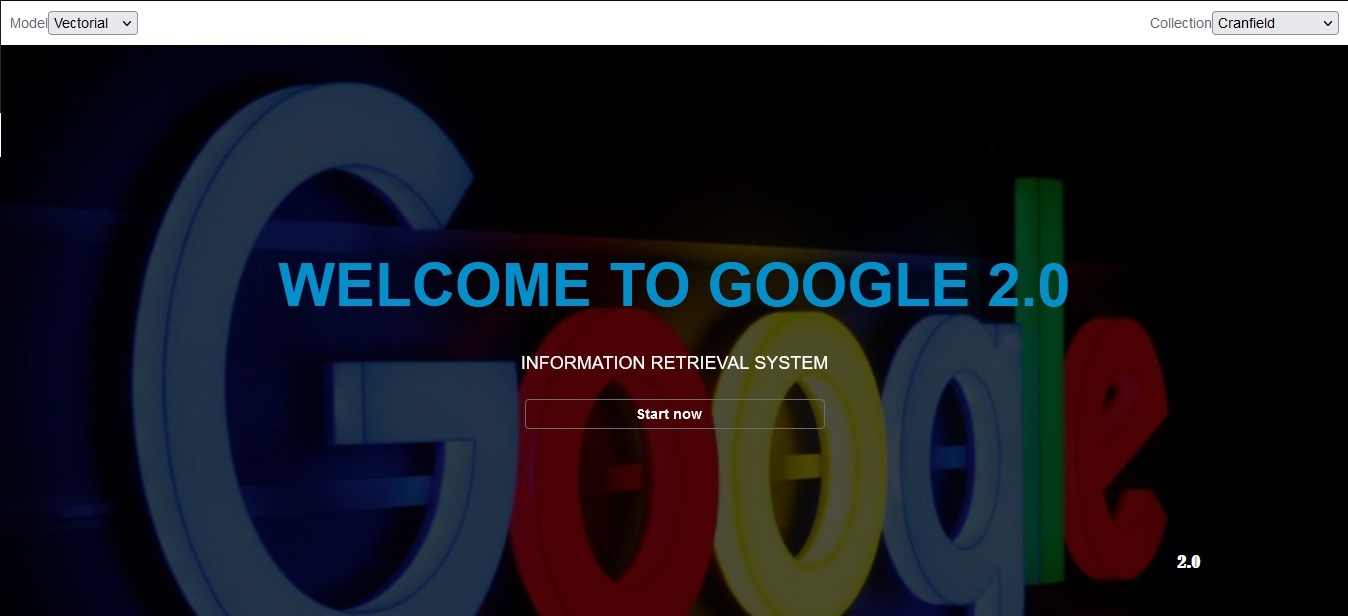
\includegraphics[scale=0.4]{img/portada.jpg}

Donde en la esquina superior derecha se podr\'a escoger para procesar entre varias colecciones de documentos, que se encuentran en la carpeta "static/collections". Para crear una nueva colecci\'on simplemente se debe crear una nueva carpeta en dicho directorio, y a\~nadirle los archivos que formar\'an parte de la colecci\'on. Luego podr\'a escoger la nueva colecci\'on desde la aplicaci\'on.

En la esquina superior izquierda se podr\'a escoger el modelo con el cual se desea procesar la colecci\'on.

Una vez definidos los par\'ametros anteriores mediante el bot\'on \textit{Start now} comienza el procesamiento de la colecci\'on seleccionada con el modelo escogido. Cuando la colecci\'on se haya procesado se muestra la siguiente pantalla:\\

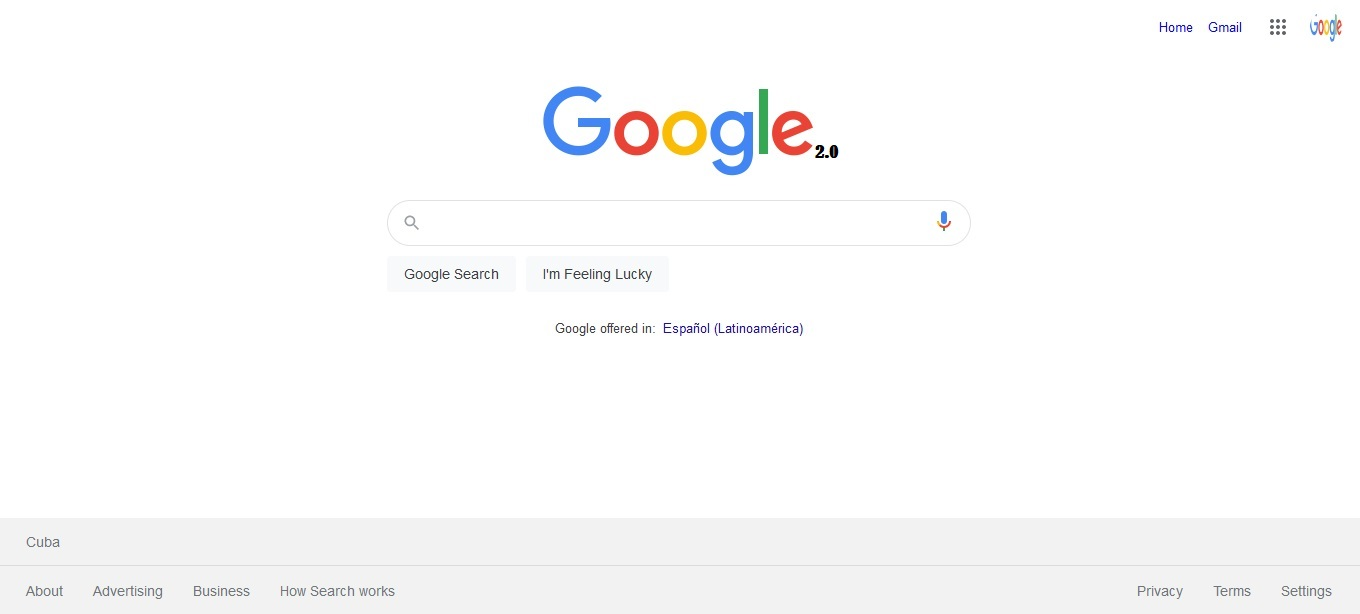
\includegraphics[scale=0.4]{img/barra_busqueda.jpg}

En la barra de b\'usqueda se inserta la consulta de inter\'es para el usuario y se da enter para obtener los resultados. El bot\'on home regresa a la pantalla de portada. Los resultados se muestran de la siguiente manera:\\

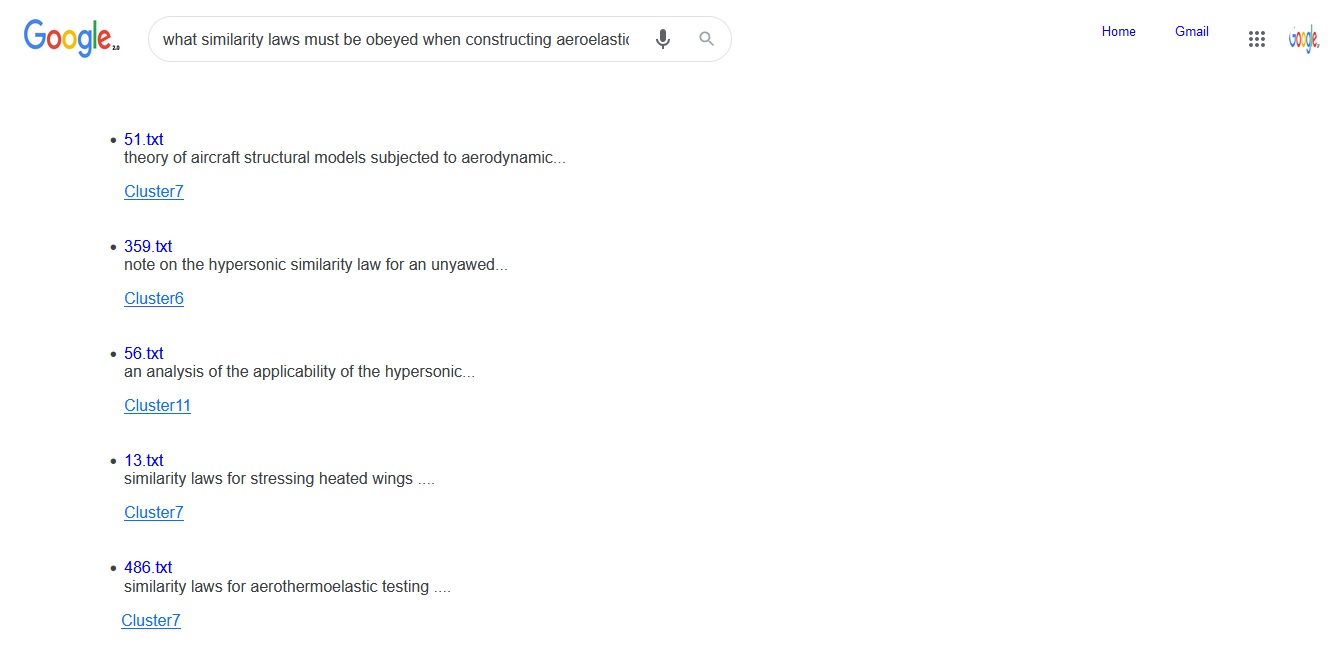
\includegraphics[scale=0.4]{img/clusters.jpg}

Si se da click encima del nombre del documento se muestra su contenido, adem\'as, se observa que cada documento tiene asociado un t\'opico o tema (cluster) y, dando click sobre este, se listan todos los documentos relacionados con el tema, por si el usuario tiene inter\'es por alg\'un otro documento de este t\'opico. Adicionalmente, se muestra la primera l\'inea de cada documento devuelto como resultado de la consulta.

Para ejecutar la aplicaci\'on es necesario tener un navegador web. Junto a este informe se provee un .exe que ejecuta la aplicaci\'on. Se debe aclarar que, para cerrar la aplicaci\'on y que no se quede corriendo el servidor en el puerto, se debe salir presionando Ctrl+c en la consola que se abre junto a la aplicaci\'on.



\section{Evaluaci\'on del sistema}
\qquad Para evaluar un sistema es necesario utilizar colecciones de prueba, las cuales contienen los documentos y, adem\'as, informaci\'on acerca de los documentos relevantes para un conjunto de consultas. Las pruebas utlizadas para evaluar el presente sistema son las colecciones de Cranfield y Medline, que se encuentran en \textbf{code/collections/}. El m\'odulo \texttt{evaluation.py} se encarga de procesar los documentos y las consultas de cada una de las colecciones antes mencionadas, devolviendo las m\'etricas estudiadas durante el curso de SRI, que nos permitir\'an evaluar el sistema implementado.

Es importante aclarar que, dado el tama\~no que presentan las colecciones, el proceso de evaluaci\'on se demora considerablente, ya que procesa los documentos para dos modelos, adem\'as de un gran n\'umero de consultas.

\subsection{M\'etricas utilizadas}
\qquad En [5] se proponen varias m\'etricas para evaluar un sistema de recuperaci\'on de la informaci\'on y, para un mejor entendimiento de sus f\'ormulas se aclaran las siguientes notaciones:
\begin{enumerate}
\item \textbf{REL} conjunto de documentos relevantes
\item \textbf{REC} conjunto de documentos recuperados
\item \textbf{RR} conjunto de documentos relevantes recuperados
\item \textbf{NN} conjunto de documentos no relevantes no recuperados
\item \textbf{RI} conjunto de documentos recuperados irrelevantes
\item \textbf{NR} conjunto de documentos no recuperados relevantes
\end{enumerate} [5]


Las medidas usadas son las siguientes:
\begin{itemize}
\item Precisi\'on. $$P = \frac{|RR|}{|RR \cup RI|} = \frac{|RR|}{|REC|}$$ Esta medida eval\'ua la consulta de acuerdo a los documentos relevantes que se recuperan[5]. Despu\'ees de tener los documentos que fueron recuperados en la consulta, se buscan cu\'ales son relevantes con ayuda de la informaci\'on brindada por la colecci\'on, y teniendo esto, se aplica la f\'ormula. Este proceso se realiz\'o para cada consulta de la colecci\'on y los resultados obtenidos fueron promediados.

\item Recobrado. $$R = \frac{|RR|}{|RR \cup RN|} = \frac{|RR|}{|REL|}$$ fracci\'on de los documentos relevantes que fueron recuperados[5]. Con ayuda de la informaci\'on que brinda la colecci\'on se buscan los documentos relevantes para la consulta, teniendo ya los documentos recuperados se va analizando de estos, cu\'ales son relevantes, e igualmente se aplica la f\'ormula. El proceso se realiza para cada consulta de la colecci\'on y los resultados obtenidos se promedian.

\item Medida F. $$F = \frac{(1+\beta^2)PR}{\beta^2P + R} = \frac{(1+\beta^2)}{\frac{1}{P} + \frac{\beta^2}{R}}$$ enfatiza la precisi\'on sobre el recobrado o viceversa[5]. Igualmente, el proceso se realiza para cada consulta de la colecci\'on y los resultados obtenidos se promedian.

\item Medida F1. $$F1 = \frac{2PR}{P+R} = \frac{2}{\frac{1}{P} + \frac{1}{R}}$$ armoniza precisi\'on y recobrado teniendo en cuenta a ambos.[5] Para su c\'alculo se us\'o la precisi\'on y el recobrado, previamente calculados, y se aplic\'o la
f\'ormula. Igualmente, el proceso se realiza para cada consulta de la colecci\'on y los resultados obtenidos se promedian.

\item R-Precisi\'on. $$P_R = \frac{|RR|_R}{|RR \cup RI|_R} = \frac{|RR|_R}{|REC|_R}$$ es el ranking de documentos relevantes a una consulta para la cual existen R documentos relevantes[5]. Para su c\'alculo se seleccionaron los primeros R documentos recuperados y de estos se vieron cu\'ales son relevantes, de acuerdo a la informaci\'on que brinda la colecci\'on y se aplica la f\'ormula. El proceso se realiza para cada consulta de la colecci\'on y los resultados obtenidos se promedian.

\item Fallout $$Fallout = \frac{|RI|}{|RI \cup NI|} = \frac{|RI|}{|I|}$$ tiene en cuenta la cantidad de documentos irrelevantes
y el ranking [5]. Se puede calcular la cardinalidad del conjunto de los documentos recuperados irrelevantes con la diferencia de los documentos recuperados y de los recuperados relevantes. Por otro lado, con la diferencia del total de documentos y los documentos relevantes, se tiene el conjunto de los documentos irrelevantes; luego, se aplica la f\'ormula y se repite el
proceso para cada consulta de la colecci\'on y los resultados se promedian.
\end{itemize}


\subsection{An\'alisis de los resultados obtenidos}
\qquad Para mostrar los resultados de la evaluaci\'on del m\'etodo booleano y el vectorial en dos escenarios distintos, se debe abrir la consola en el directorio del proyecto y ejecutar \texttt{python evaluation.py} Esto ejecutar\'a ambos modelos sobre las colecciones de Cranfield y Medline[6], mostrando el c\'alculo de las medidas de evaluaci\'on abordadas en la secci\'on anterior. En el caso de las medidas que tienen en cuenta el ranking, se tomar\'an los primeros 10 documentos.

En un primer escenario, la colecci\'on Cranfield, se cuenta con 1400 documentos y 225 consultas, en la que, luego de aplicar el modelo vectorial se arribaron a los siguientes resultados:

Si se fija un umbral de 0.08:\\\\
\texttt{
Precision Average: 0.1094814814814814815 \\
Recall Average: 0.644597701149425287 \\
F (beta = 0) Average: 0.1094814814814814 \\
F1 Average: 0.18602870470039468962 \\
R-precision Average: 0.250044444444444447 \\
Fallout Average: 0.031425460436968326 \\\\
}

Como se observa, se tiene una precisi\'on baja y un recobrado relativamente alto, lo cual puede estar dado porque se devuelven muchos documentos como resultado a las consultas. Si se prueba con un umbral m\'as elevado, 0.15, se tiene que\\\\
\texttt{
Precision Average: 0.17667238645741274 \\
Recall Average: 0.081436161800807733 \\
F (beta = 0) Average: 0.17667238645741 \\
F1 Average: 0.0989109335636531973 \\
R-precision Average: 0.0853634000283629 \\
Fallout Average: 0.0128324467540477802 \\\\
}

En este caso los valores son bajos, lo que puede estar dado porque se devuelven muy pocos documentos como resultado a consultas. Si se fija un umbral que se encuentre en el centro de los dos valores, los resultados deben mejorar. Se debe buscar un equilibrio en el que no sea abrumadora la cantidad de documentos que se devuelven, ni muy poca. Si se ejecutan las evaluaciones con un umbral del 0.11 se obtiene:\\\\
\texttt{
Precision Average: 0.57987467891626214 \\
Recall Average: 0.439855042462559 \\
F (beta = 0) Average: 0.57987467891626 \\
F1 Average: 0.45654982088860464 \\
R-precision Average: 0.5628909908643447 \\
Fallout Average: 0.005557089650605272 \\\\
}

Se observa que la precisi\'on y el recobrado oscilan sobre los mismos valores, entre 0.4 y 0.6, los cuales son valores buenos, que indican que el sistema devuelve los resultados esperados. Las otras medidas tambi\'en son buenas, lo que ratifica que lo expresado anteriormente.\\

Si en este escenario aplicamos el modelo booleano, con un l\'imite de documentos resultantes de 40, se obtiene que:\\\\
\texttt{
Precision Average: 0.0966402407556727 \\
Recall Average: 0.205010479814852074 \\
F (beta = 0) Average: 0.0966402407556 \\
F1 Average: 0.12414552678756908 \\
R-precision Average: 0.3022575531659254 \\
Fallout Average: 0.05332300012708674 \\\\
}
Se observa un muy bajo valor de precisi\'on, lo que puede estar dado por la cantidad de documentos que se devuelven. El recobrado es relativamente bajo, as\'i como las otras medidas. Se intentar\'a ahora con un valor de 10 documentos resultantes como l\'imite.\\\\
\texttt{
Precision Average: 0.115019878494544 \\
Recall Average: 0.035371411909860904 \\
F (beta = 0) Average: 0.115019878494544 \\
F1 Average: 0.0471018653142009 \\
R-precision Average: 0.056069958150249385 \\
Fallout Average: 0.021353375534192 \\\\
}

En este caso las medidas son muy bajas, por lo que el modelo no esta devolviendo los resultados esperados. Si se fija un valor de 25 documentos como l\'imite, se obtiene:\\\\
\texttt{
Precision Average: 0.43725477494339827 \\
Recall Average: 0.38781951274405562 \\
F (beta = 0) Average: 0.43725477494339827 \\
F1 Average: 0.409038370028197194 \\
R-precision Average: 0.41934086302500142 \\
Fallout Average: 0.007953313599142427 \\\\
}

En este caso las medidas tienen valores relativamente altos, siendo la precisi\'on la m\'as elevada. Estos valores no est\'an mal, si bien no son ideales, indican que el sistema, con el modelo booleano, devuelve algunos resultados que satisfacen las necesidades del usuario.\\\\

Si ejecutamos el sistema sobre la colecci\'on de Medline, se tiene que, para el modelo vectorial implementado, se obtienen los siguientes resultados:

Si se fija un umbral de 0.08\\\\
\texttt{
Precision Average: 0.095555400507532 \\
Recall Average: 0.61641704263402854 \\
F (beta = 0) Average: 0.095555400507532 \\
F1 Average: 0.0621209195982305 \\
R-precision Average: 0.16541951566913747 \\
Fallout Average: 0.06254018467969548 \\\\
}
Como se observa, se tiene una precisi\'on baja y un recobrado relativamente alto, lo cual puede estar dado porque se devuelven muchos documentos como resultado a las consultas. Si se prueba con un umbral m\'as elevado, 0.15, se tiene que\\\\
\texttt{
Precision Average: 0.260371458963389 \\
Recall Average: 0.0642323967561534 \\
F (beta = 0) Average: 0.260371458963 \\
F1 Average: 0.103046485092519685 \\
R-precision Average: 0.07570631341196 \\
Fallout Average: 0.0457742784840535 \\\\
}

En este caso los valores son bajos, lo que puede estar dado porque se devuelven muy pocos documentos como resultado a consultas. Si se fija un umbral que se encuentre en el centro de los dos valores, los resultados deben mejorar. Se debe buscar un equilibrio en el que no sea abrumadora la cantidad de documentos que se devuelven, ni muy poca. Si se ejecutan las evaluaciones con un umbral del 0.11 se obtiene:\\\\
\texttt{
Precision Average: 0.530371458963389 \\
Recall Average: 0.5042323967561534 \\
F (beta = 0) Average: 0.5303714589633 \\
F1 Average: 0.63046485092519685 \\
R-precision Average: 0.0757063134119 \\
Fallout Average: 0.0057742784840535 \\\\
}

En este caso los resultados son muy buenos, se obtuvo una precisi\'on alta, al igual que el recobrado. Lo que indica que la mayor\'ia de los documentos recuperados fueron relevantes. El resto de las medidas tambi\'en fueron muy buenas.\\

Si en este escenario aplicamos el modelo booleano, con un l\'imite de documentos resultantes de 40, se obtiene que:\\\\
\texttt{
Precision Average: 0.07711344455390836 \\
Recall Average: 0.175527036341846 \\
F (beta = 0) Average: 0.07711344455390836 \\
F1 Average: 0.10809409640170624 \\
R-precision Average: 0.2863479703627805 \\
Fallout Average: 0.07002101566858976 \\\\
}

En esta ocasi\'on se devuelven demasiados documentos, lo cual se ve reflejado en los valores anteriores. Se observa un muy bajo valor de precisi\'on, lo que puede estar dado por la cantidad de documentos que se devuelven. El recobrado es relativamente bajo, as\'i como las otras medidas. Se intentar\'a ahora con un valor de 10 documentos resultantes como l\'imite.\\\\
\texttt{
Precision Average: 0.157913591314895 \\
Recall Average: 0.0526228257992206 \\
F (beta = 0) Average: 0.157913591314895 \\
F1 Average: 0.0780621041862924 \\
R-precision Average: 0.06366182045593243 \\
Fallout Average: 0.03506911904879048 \\\\
}

En este caso las medidas son muy bajas, lo que puede venir dado por la poca cantidad de documentos que devuelve el modelo, adem\'as, no est\'a devolviendo los resultados esperados. Si se fija un valor de 25 documentos como l\'imite, se obtiene:\\\\
\texttt{
Precision Average: 0.4075456344647778 \\
Recall Average: 0.3685410468103969 \\
F (beta = 0) Average: 0.4075456344647778 \\
F1 Average: 0.3870973090372418 \\
R-precision Average: 0.3970972693403497 \\
Fallout Average: 0.0868155098017147 \\\\
}

Finalmente, el modelo booleano en este escenario se comporta de una forma relativamente bien. Las medidas tienen valores relativamente altos, siendo la precisi\'on la m\'as elevada. Estos valores no est\'an mal, si bien no son ideales, indican que el sistema, con el modelo booleano, devuelve algunos resultados que satisfacen las necesidades del usuario en este escenario.

\section{Ventajas y desventajas del sistema}
\qquad El sistema implementado presenta varias ventajas, entre las que se pueden mencionar que las m\'etricas usadas en la secci\'on anterior para la evaluaci\'on del sistema dan resultados favorables. Devuelve resultados satisfactorios a las necesidades que el usuario define a trav\'es de consultas. Adem\'as, presenta funcionalidades como expansi\'on de consulta, agrupamiento de documentos por t\'opicos o clustering y una interfaz de usuario amigable para la inserci\'on de las consultas y mostrar los resultados.

Como desventaja se puede decir que el sistema solo trabaja localmente en una colecci\'on escogida por el usuario, adem\'as, el procesamiento de documentos demora un poco, sobre todo en colecciones grandes con documentos extensos.
 
\section{Conclusiones}
\qquad El sistema implementado presenta buenos resultados. Realizar un sistema de recuperaci\'on de informaci\'on es un proceso trabajoso que lleva asociado un proceso de an\'alisis y estudio. A\'un as\'i el presente sistema responde de manera positiva en los escenarios donde se realiz\'o el proceso de evaluaci\'on. 

En ambos escenarios, con los par\'ametros indicados, el sistema obtuvo buenas m\'etricas. Lo que quiere decir que procesa los documentos y la consulta del usuario de manera satisfactoria, devolviendo resutados de inter\'es para el usuario. El modelo vectorial demostr\'o ser mejor que el booleano en ambos escenarios, lo que puede venir dado porque los documentos no ten\'ian la consulta de forma expl\'icita en su texto, a pesar de que la expansi\'on de consulta ayuda mucho al modelo booleano a devolver mejores resultados, no logr\'o superar al otro modelo implementado. Ambos modelos mostraron patrones similares en ambos escenarios, dando resultados favorables. 

\section{Recomendaciones y trabajo futuro}
\qquad Al sistema se le pueden a\~nadir un conjunto de mejoras para que funcione de manera \'optima, y agregar nuevas funcionalidades para devolver mejores resultados, entre las que se encuentran:
\begin{itemize}
\item A\~nadir retroalimentaci\'on.
\item Optimizar el procesamiento de documentos
\item A\~nadir crawling como sistema de recuperaci\'on en la web
\end{itemize}






\section{Bibliograf\'ia}
$[1]$ http://sedici.unlp.edu.ar/bitstream/handle/ 10915/43840/ Documento\_completo.pdf? sequence=1\&isAllowed=y\\\\
$[2]$ Conferencias 2 y 3 SRI para la carrera de Ciencia de la Computaci\'on, Universidad de La Habana. Curso 2022\\\\ 
$[3]$ https://bid.ub.edu/04figue2.htm\\\\
$[4]$ Conferencia 2 SRI para la carrera de Ciencia de la Computaci\'on, Universidad de La Habana. Curso 2022\\\\
$[5]$ Conferencia 4 SRI para la carrera de Ciencia de la Computaci\'on, Universidad de La Habana. Curso 2022\\\\
$[6]$ http://ir.dcs.gla.ac.uk/resources/test\_collections/

%\end{multicols}{2}
\end{document}